\newcommand{\defaultparindent}{\parindent}
\setlength{\parindent}{0pt}				% \noindent partout
% \parindent in one-column documents is :
% 15pt when the default text size is 10pt,
% 17pt for 11pt,
% and 1.5em for 12pt.
% In two-column documents it is 1em

%\begin{center}
%\begin{tabular}{p{5cm} p{11cm}}
%\textbf{Commandes étudiées :} & \texttt{sh}, \texttt{bash}, \texttt{man}, \texttt{ls}, \texttt{mkdir}, \texttt{touch}, \texttt{chmod}, \texttt{mv}, \texttt{rm}, \texttt{rmdir}, \texttt{cat}, \texttt{file}, \texttt{whereis}, \texttt{which}\\

%\textbf{Builtins étudiées :} & \texttt{pwd}, \texttt{cd}, \texttt{exit}, \texttt{logout}, \texttt{echo}, \texttt{umask}, \texttt{type}, \texttt{>}, \texttt{>{}>}, \texttt{<}, \texttt{<{}<}, \texttt{|}\\

%\textbf{Notions étudiées :} & Tableaux, Pointeurs, Piles\\
%\end{tabular}
%\end{center}

\textbf{Notions étudiées :} Tableaux, Pointeurs, Piles\\

%\bigskip

\subsection{Rappel sur les piles}

\bigskip

Les \textbf{piles}, ou \textbf{stacks} en anglais, sont des structures visant à stocker les données dans l'ordre d'arrivée, mais ne permettant leur récupération uniquement dans l'ordre inverse.
Dans une pile, on ne peut accéder qu'à la dernière donnée stockée, celle se situant au \textit{sommet} de la pile.
Ces structures sont aussi appelées \textbf{LIFO} (\textit{Last In First Out}).\\

\begin{center}
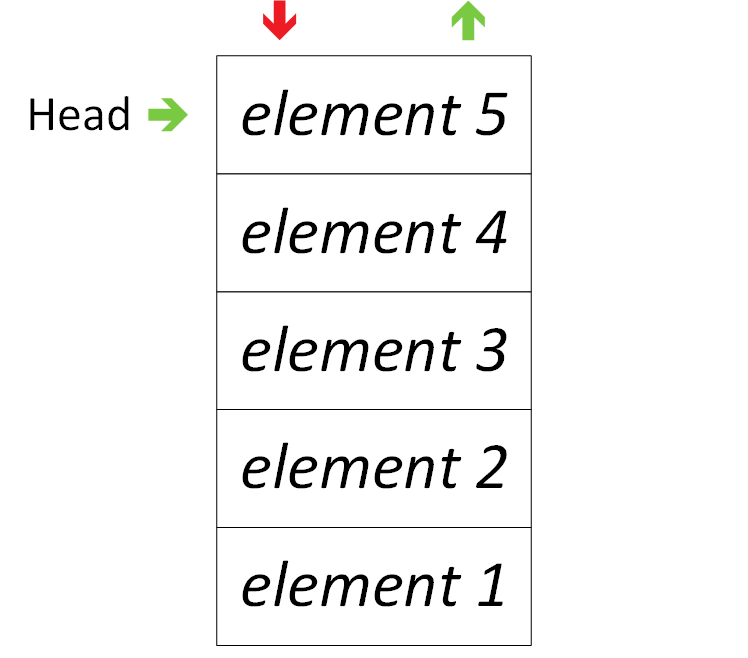
\includegraphics[scale=0.75]{Cours/Piles_1_Structure_Generale_centered.png}
\end{center}

\smallskip

Deux opérations permettent d'utiliser une pile :
\begin{itemize}
\item \TTBF{PUSH} : permettant d'\textit{empiler} une donnée supplémentaire dans la pile
\item \TTBF{POP} : permettant de \textit{dépiler} une donnée depuis la pile
\end{itemize}
On ajoute donc une donnée en l'empilant avec un \TTBF{PUSH}, et il est possible de directement y accéder, car elle est au sommet de la pile.
À l'inverse, pour accéder à une donnée tout au fond de la pile, il est nécessaire de dépiler autant d'éléments que nécessaire avec un \TTBF{POP}.\\

Voici un exemple où l'on crée une pile, puis on empile successivement $ 42 $, $ 5 $, et $ 13 $, puis, on dépile une fois (pour récupérer $ 13 $), et enfin, on empile successivement $ 37 $, $ 10 $, $ 24 $.\\

\begin{center}
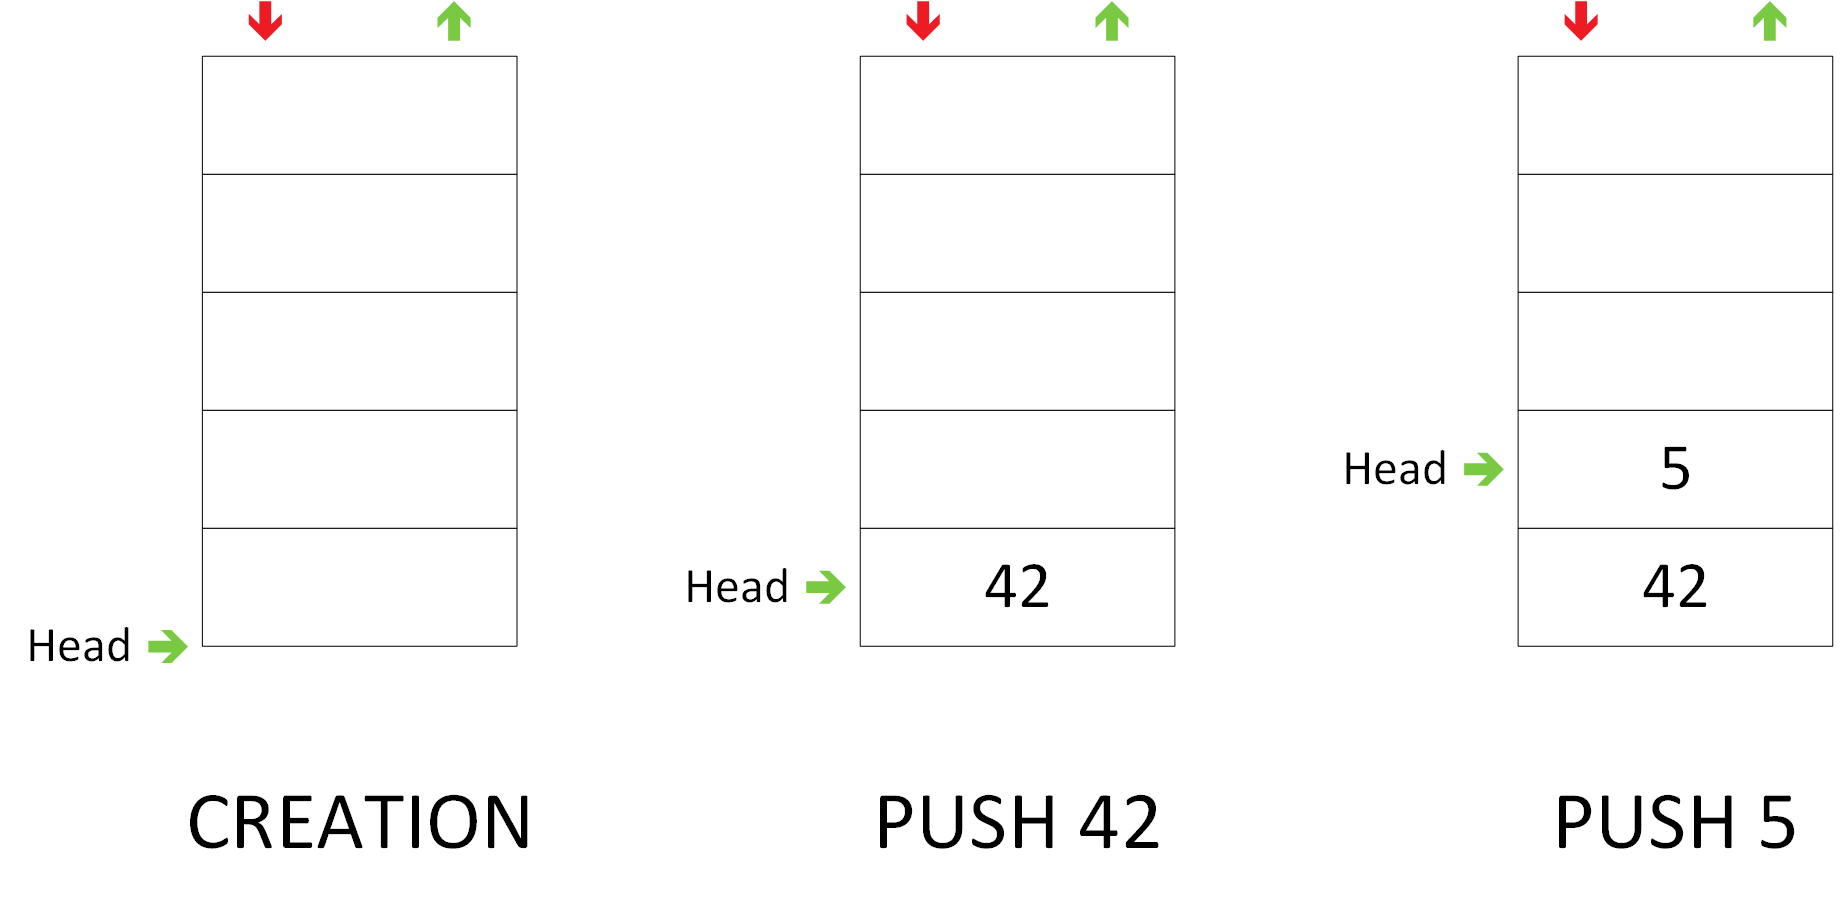
\includegraphics[scale=0.5]{Cours/Piles_2_Structure_Generale_Usage_pack_1.png}
\end{center}

\begin{center}
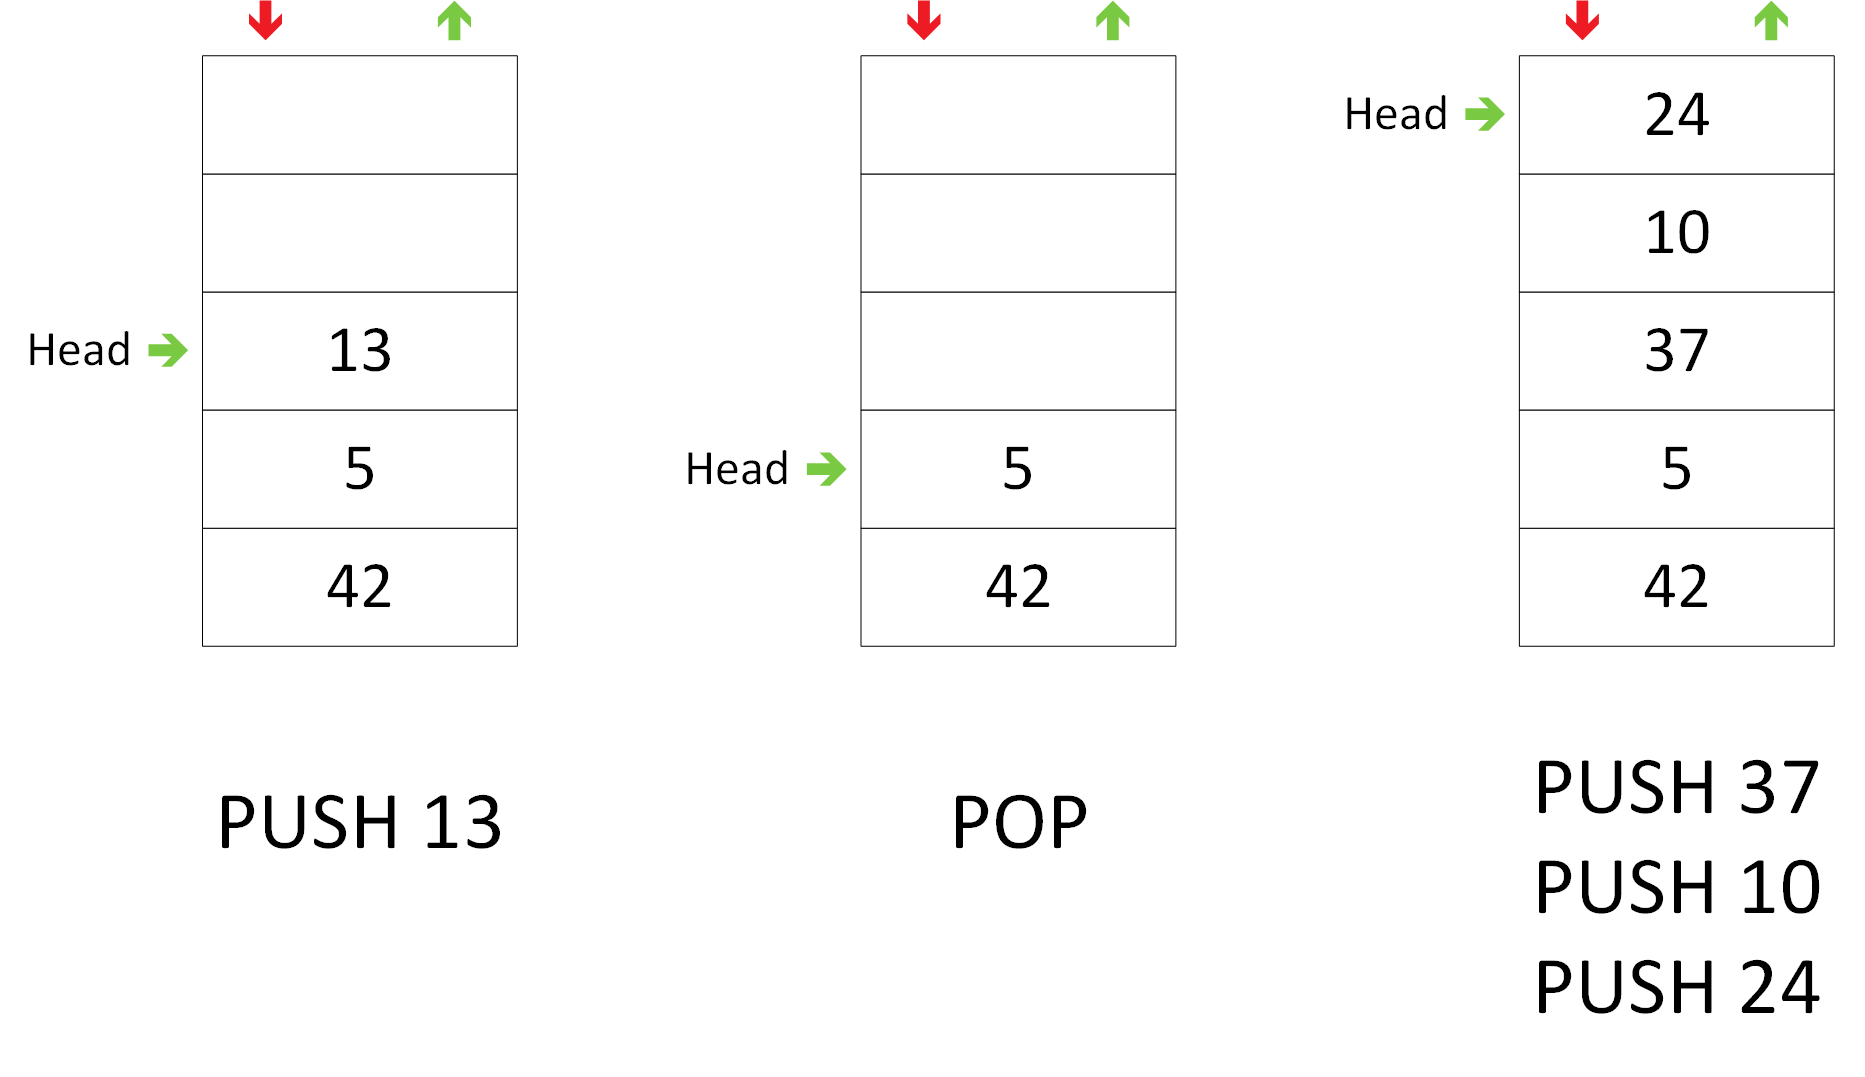
\includegraphics[scale=0.5]{Cours/Piles_2_Structure_Generale_Usage_pack_2.png}
\end{center}

\smallskip

Les piles, et surtout la contrainte d'accès aux objets, sont couramment utilisées : un camion de livraison sera d'abord rempli avec les paquets à livrer en dernier/le camion sera rempli dans l'ordre inverse de livraison (on accède d'abord aux derniers éléments chargés).

En informatique, on utilisera les piles dans certains \textit{parsers} (analyse grammaticale) pour connaître en premier l'opérateur à exécuter (opérateur binaire ? unaire ?) et dépiler par la suite le nombre exact de paramètres.
La \textit{pile d'appels} est également une convention fondamentale partagée par les processeurs et les systèmes d'exploitation permettant de passer des paramètres (et d'autres informations de contexte) aux fonctions appelées par les programmes, ou en cas d'interruption pour sauvegarder l'adresse de l'instruction qui était en cours d'exécution.\\

Afin d'implémenter une pile, il est donc nécessaire d'avoir un espace de stockage ordonné (un tableau numéroté ou une liste chaînée), et un indicateur de l'élément en haut de la pile.
Nous allons maintenant voir comment implémenter une pile avec des listes chaînées et un tableau de taille fixe.

\bigskip

%%%%%%%%%%%%%%%%%%%%%%%%%%%%%%%%%%%%%%%%%%%%%%%%%%%%%%%%%%%%
%%%%%%%%%%%%%%%%%%%%%%%%%%%%%%%%%%%%%%%%%%%%%%%%%%%%%%%%%%%%
%%%%%%%%%%%%%%%%%%%%%%%%%%%%%%%%%%%%%%%%%%%%%%%%%%%%%%%%%%%%

\subsection{Piles : implémentation avec des listes chaînées}

\bigskip

Une implémentation à l'aide d'une liste chaînée permet d'exploiter la mémoire et d'être donc beaucoup plus flexible en terme de nombre maximum d'éléments.
Le schéma suivant illustre une pile sous forme de liste chaînée en mémoire :\\

\begin{center}
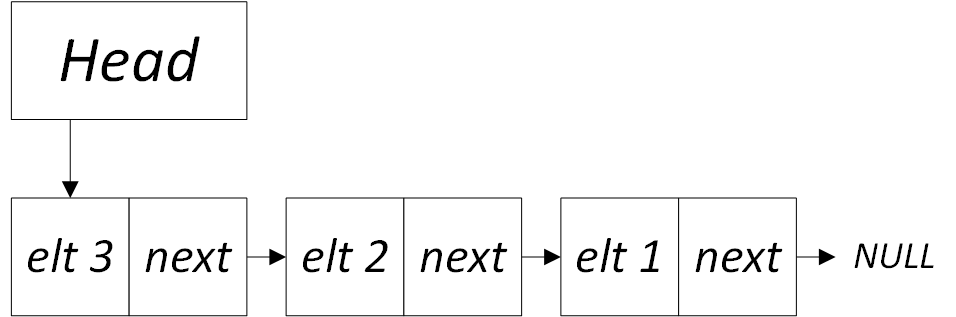
\includegraphics[scale=0.75]{Cours/Piles_3_Liste_Chainee_Structure_cas_general.png}
\end{center}

\smallskip

On y retrouve plusieurs fois la structure typique des listes chaînées (un élément et un pointeur vers l'élément suivant), ainsi qu'un pointeur indiquant le sommet de la pile (\textit{head} dans notre cas).

L'unique cas particulier concerne une pile vide : le pointeur de sommet vaut dans ce cas \TTBF{NULL}.
Il s'agit également de l'état dans lequel se trouve une pile vidée ou nouvellement créée.\\

\begin{center}
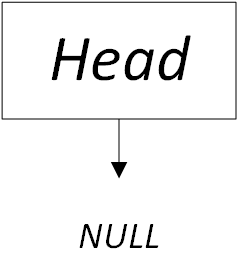
\includegraphics[scale=0.75]{Cours/Piles_3_Liste_Chainee_Structure_cas_vide.png}
\end{center}

\smallskip

L'exemple suivant montre l'évolution d'une pile au fur et à mesure des ajouts (empiler / \TTBF{PUSH}) et suppressions (dépiler / \TTBF{POP}).\\

\begin{center}
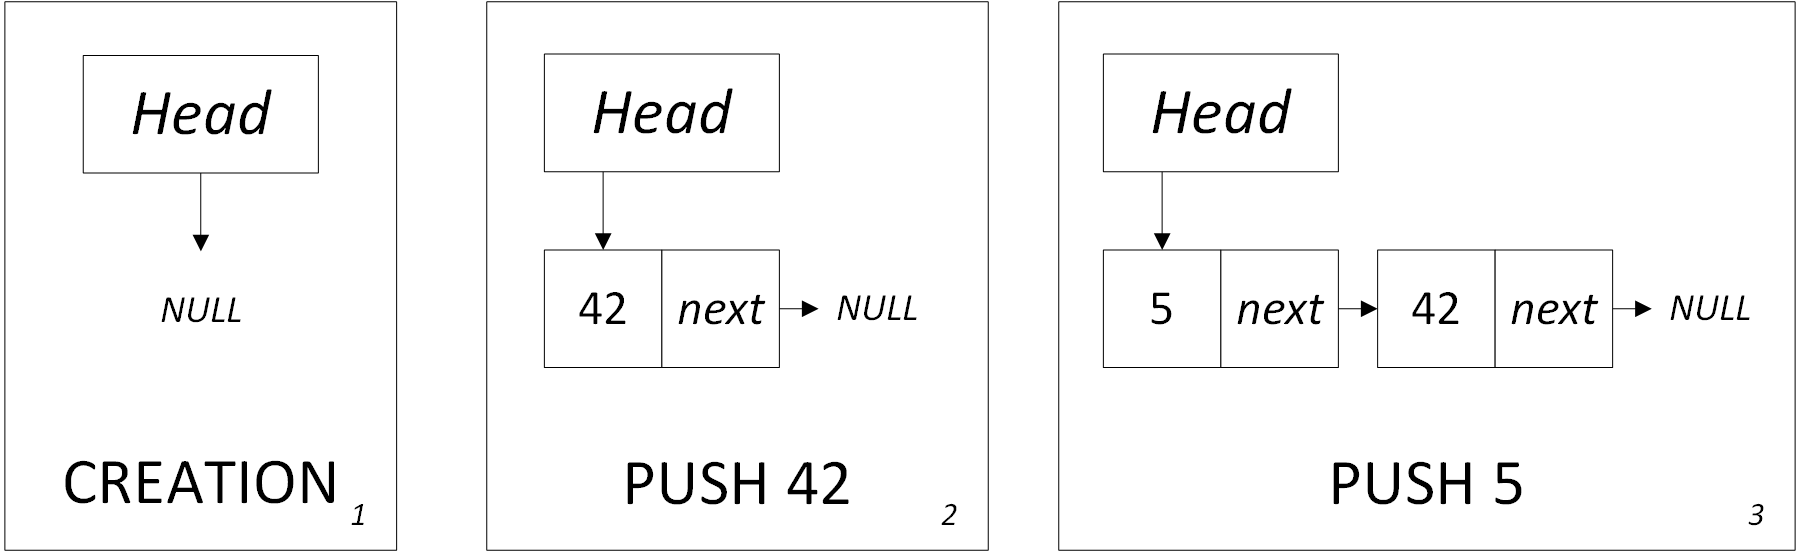
\includegraphics[scale=0.65]{Cours/Piles_4_Liste_Chainee_Usage_pack_1.png}
\end{center}

\begin{center}
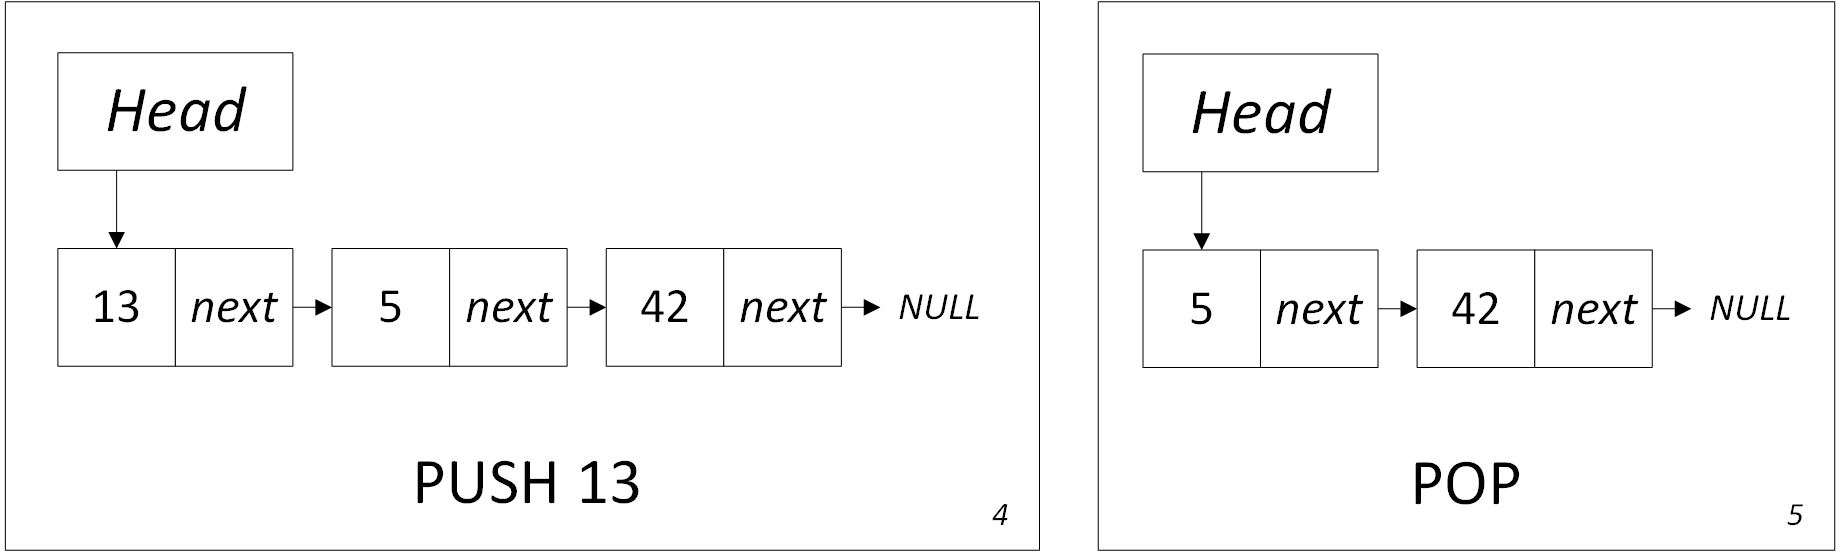
\includegraphics[scale=0.65]{Cours/Piles_4_Liste_Chainee_Usage_pack_2.png}
\end{center}

\smallskip

Les principales opérations se résument ainsi :
\begin{itemize}
\item Création : on alloue en mémoire la structure générale de la pile, et on fixe le sommet de la pile à \TTBF{NULL}.
\item Empiler : on alloue en mémoire un nouvel élément dont le pointeur \textit{next} pointe vers l'actuel élément au sommet de la pile, puis, on met à jour le pointeur de sommet de la pile vers l'adresse de ce nouvel élément.
\item Dépiler : si la pile est vide, on retourne une erreur, sinon, on récupère tout d'abord l'adresse de l'élément suivant celui au sommet, puis, on libère l'élément au sommet, puis, on met à jour le pointeur de sommet de la pile vers l'adresse de l'élément suivant.
\item Vider : on dépile successivement tous les éléments jusqu'à obtenir un sommet à \TTBF{NULL}.
\item Sommet : on renvoie le contenu de l'élément au sommet de la pile.
\end{itemize}

\bigskip

%%%%%%%%%%%%%%%%%%%%%%%%%%%%%%%%%%%%%%%%%%%%%%%%%%%%%%%%%%%%
%%%%%%%%%%%%%%%%%%%%%%%%%%%%%%%%%%%%%%%%%%%%%%%%%%%%%%%%%%%%
%%%%%%%%%%%%%%%%%%%%%%%%%%%%%%%%%%%%%%%%%%%%%%%%%%%%%%%%%%%%

\subsection{Piles : implémentation avec un tableau de taille fixe}

\bigskip

Une implémentation avec un tableau de taille fixe impose cette fois une limitation : la pile aura une taille maximale, et on peut refuser l'ajout d'un élément si la pile est déjà pleine.
La structure diffère également du fait que le tableau est alloué une seule fois lors de sa création (voire même lors de la compilation dans le cas statique).

Le schéma suivant présente la structure générale :\\

\begin{center}
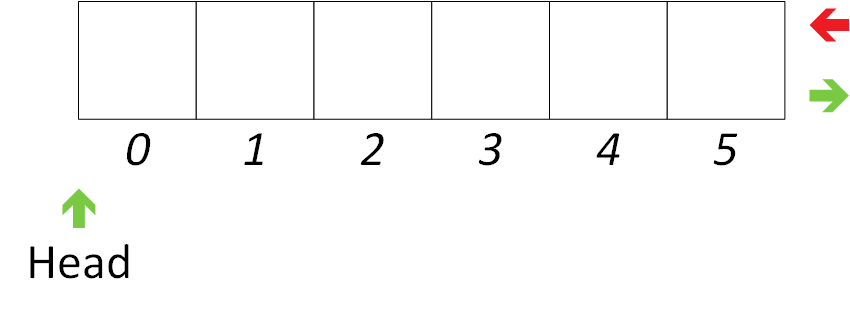
\includegraphics[scale=1]{Cours/Piles_5_Tableau_Statique_Structure.png}
\end{center}

\smallskip

On notera cette fois que plusieurs informations distinctes doivent être conservées : l'adresse du tableau, le numéro de case correspondant au sommet de la pile (\textit{head} dans notre cas), la taille du tableau (le nombre maximum d'objets pouvant être stockés), le nombre d'éléments dans le tableau.

Le schéma suivant détaille certaines informations de façon plus explicite :\\

\begin{center}
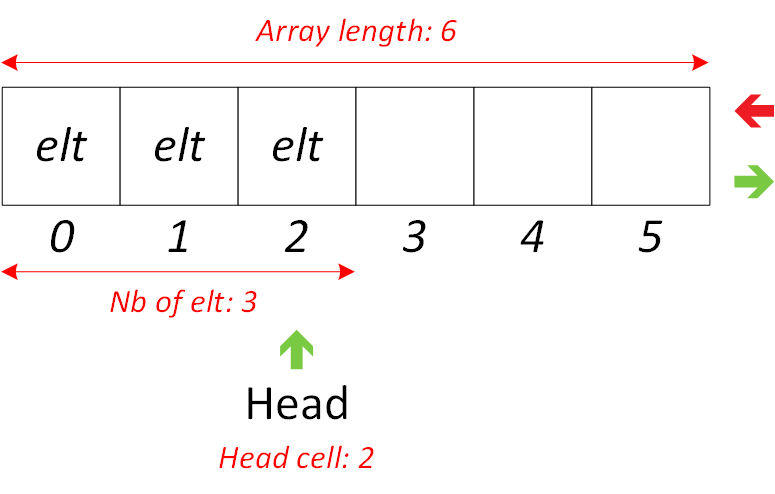
\includegraphics[scale=1]{Cours/Piles_5_Tableau_Statique_Structure_Detaillee.png}
\end{center}

\smallskip

Dans le cas d'un tableau de taille fixe, le pointeur de sommet ne peut pas utiliser la valeur \TTBF{NULL} comme indicateur de tableau vide, car cette valeur est égale à $ 0 $ (ce qui laisserait à penser que le sommet est effectivement à la case 0).
Plusieurs solutions sont possibles pour indiquer le sommet de la pile et le cas vide :

\begin{itemize}
\item On enregistre dans la structure de la pile une variable servant à compter le nombre d'éléments présents (le sommet peut donc prendre n'importe quelle valeur tant que la pile est vide).
\item On utilise un entier relatif pour indiquer le sommet, et $ -1 $ indique que la pile est vide (l'ajout d'un élément décalera le sommet à $ 0 $, c'est-à-dire la case où sera l'élément).
\item On place le sommet de la pile sur la première case non utilisée, et l'accès au premier élément se fait donc en retirant $ 1 $ au pointeur de sommet (ainsi, un sommet à la case $ 0 $ indique que la pile est vide).
Attention : dans ce cas précis, un tableau plein aura un sommet hors des cases du tableau (il ne faudra donc \textit{jamais} le déréférencer s'il atteinte une telle valeur).
\end{itemize}

\smallskip

L'exemple suivant montre l'évolution d'une pile implémentée avec un tableau fixe au fur et à mesure des ajouts (empiler / \TTBF{PUSH}) et suppressions (dépiler / \TTBF{POP}).\\

\begin{center}
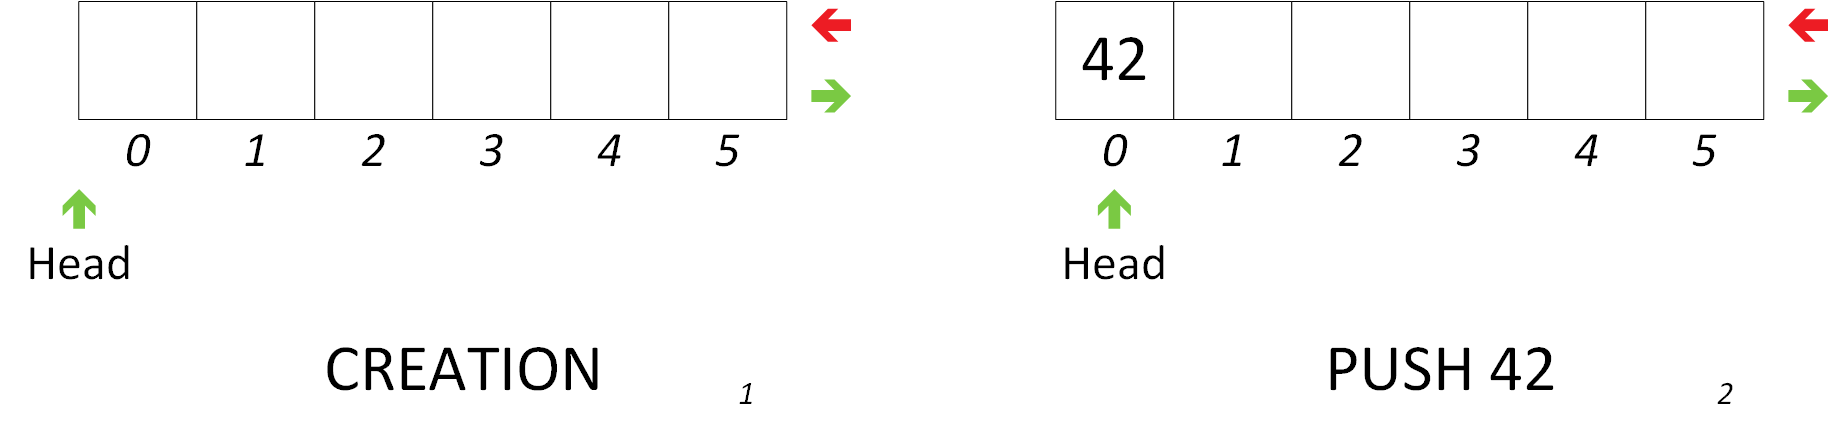
\includegraphics[scale=0.65]{Cours/Piles_6_Tableau_Statique_Usage_pack_1.png}
\end{center}

\begin{center}
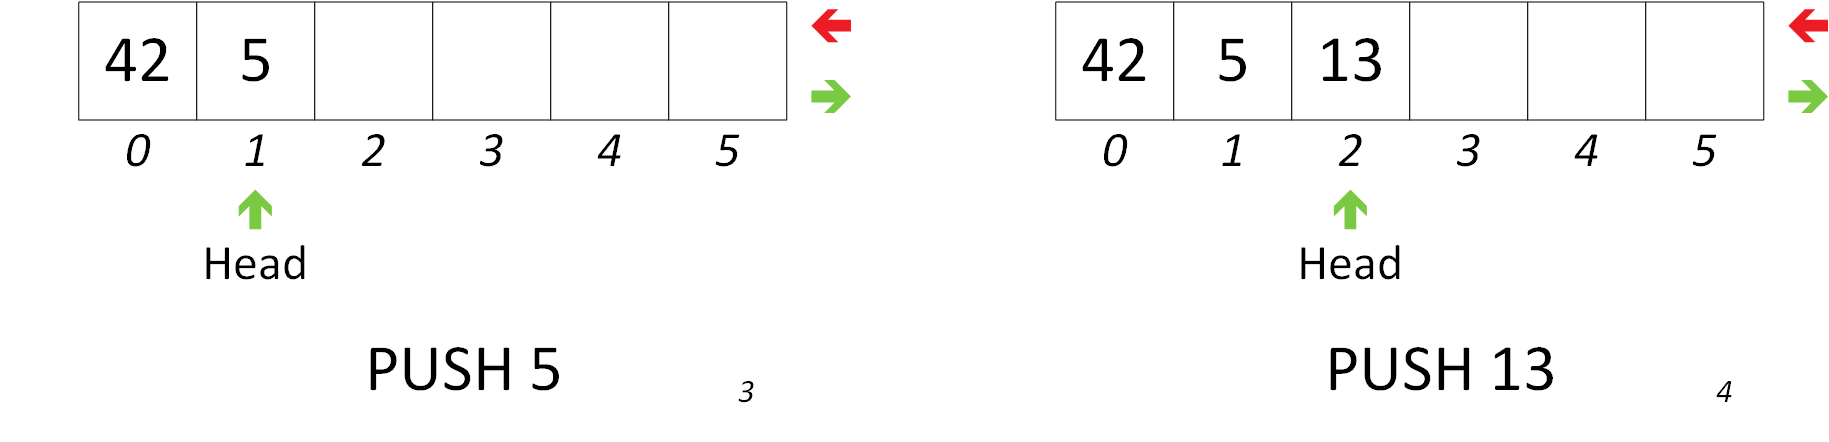
\includegraphics[scale=0.65]{Cours/Piles_6_Tableau_Statique_Usage_pack_2.png}
\end{center}

\begin{center}
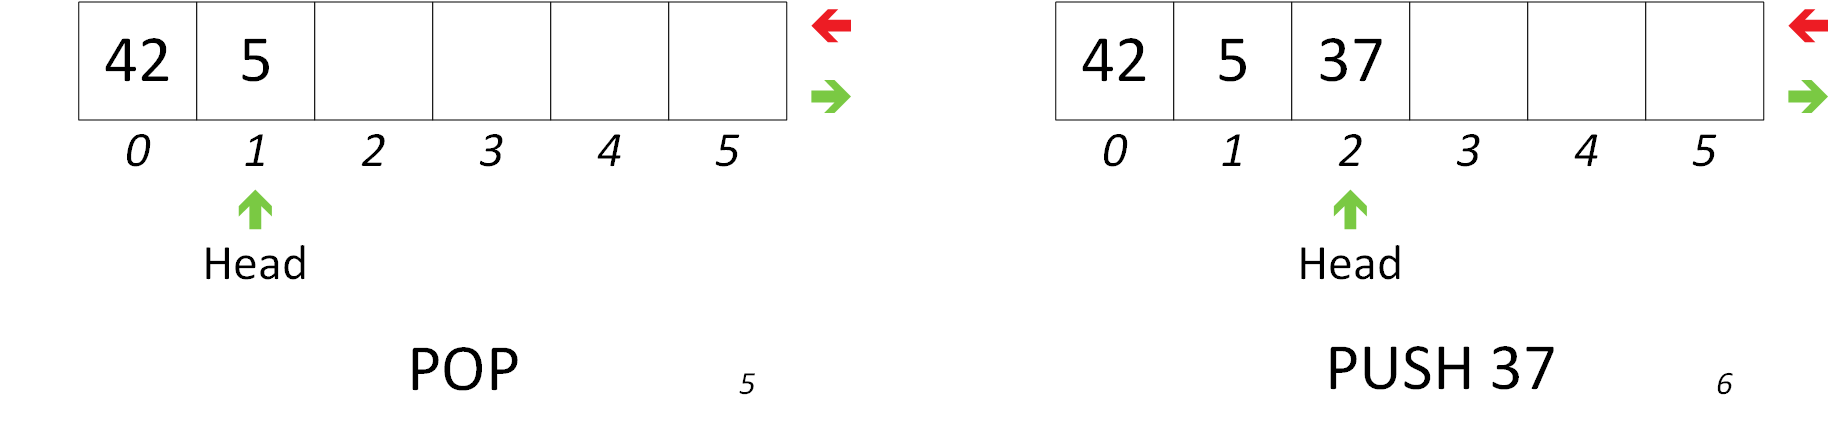
\includegraphics[scale=0.65]{Cours/Piles_6_Tableau_Statique_Usage_pack_3.png}
\end{center}

\smallskip

Les principales opérations se résument ainsi :
\begin{itemize}
\item Création : on alloue en mémoire le tableau (sauf s'il est statique), et on fixe le sommet de la pile à la valeur prévue pour démarrer ($ -1 $, $ 0 $, ou toute autre valeur choisie) [éventuellement, on met à jour le nombre d'objets dans le tableau en le fixant à $ 0 $].
\item Empiler : si le tableau est plein, on retourne une erreur, sinon, on ajoute un élément, et on décale le sommet de la pile [éventuellement, on met à jour le nombre d'objets dans le tableau].
\item Dépiler : si la pile est vide, on retourne une erreur, sinon, on réduit la valeur du sommet de la pile [éventuellement, on met à jour le nombre d'objets dans le tableau].
\item Vider : on fixe le sommet de la pile à la valeur prévue pour démarrer ($ -1 $, $ 0 $, ou toute autre valeur choisie) [éventuellement, on met à jour le nombre d'objets dans le tableau en le fixant à $ 0 $].
\item Sommet : on renvoie le dernier élément ajouté (cela dépend de comment le sommet a été implémenté !).
\end{itemize}

\setlength{\parindent}{\defaultparindent}
